% mnras_template.tex 
%
% LaTeX template for creating an MNRAS paper
%
% v3.0 released 14 May 2015
% (version numbers match those of mnras.cls)
%
% Copyright (C) Royal Astronomical Society 2015
% Authors:
% Keith T. Smith (Royal Astronomical Society)

% Change log
%
% v3.0 May 2015
%    Renamed to match the new package name
%    Version number matches mnras.cls
%    A few minor tweaks to wording
% v1.0 September 2013
%    Beta testing only - never publicly released
%    First version: a simple (ish) template for creating an MNRAS paper

%%%%%%%%%%%%%%%%%%%%%%%%%%%%%%%%%%%%%%%%%%%%%%%%%%
% Basic setup. Most papers should leave these options alone.
\documentclass[fleqn,usenatbib]{mnras}

% MNRAS is set in Times font. If you don't have this installed (most LaTeX
% installations will be fine) or prefer the old Computer Modern fonts, comment
% out the following line
\usepackage{newtxtext,newtxmath}
% Depending on your LaTeX fonts installation, you might get better results with one of these:
%\usepackage{mathptmx}
%\usepackage{txfonts}

% Use vector fonts, so it zooms properly in on-screen viewing software
% Don't change these lines unless you know what you are doing
\usepackage[T1]{fontenc}

% Allow "Thomas van Noord" and "Simon de Laguarde" and alike to be sorted by "N" and "L" etc. in the bibliography.
% Write the name in the bibliography as "\VAN{Noord}{Van}{van} Noord, Thomas"
\DeclareRobustCommand{\VAN}[3]{#2}
\let\VANthebibliography\thebibliography
\def\thebibliography{\DeclareRobustCommand{\VAN}[3]{##3}\VANthebibliography}


%%%%% AUTHORS - PLACE YOUR OWN PACKAGES HERE %%%%%

% Only include extra packages if you really need them. Common packages are:
\usepackage{graphicx}	% Including figure files
\usepackage{amsmath}	% Advanced maths commands
% \usepackage{amssymb}	% Extra maths symbols

%%%%%%%%%%%%%%%%%%%%%%%%%%%%%%%%%%%%%%%%%%%%%%%%%%

%%%%% AUTHORS - PLACE YOUR OWN COMMANDS HERE %%%%%
\usepackage{svg}

% Please keep new commands to a minimum, and use \newcommand not \def to avoid
% overwriting existing commands. Example:
%\newcommand{\pcm}{\,cm$^{-2}$}	% per cm-squared
\newcommand{\msun}{\mathcal{M}_{\sun}}
\newcommand{\orcid}[1]{\href{https://orcid.org/#1}{\includesvg[width=10pt]{orcid}}}

\newcommand{\dummyfig}[1]{
  \centering
  \fbox{
    \begin{minipage}[c][0.25\textheight][c]{\columnwidth}
      \centering{#1}
    \end{minipage}
  }
}

%%%%%%%%%%%%%%%%%%%%%%%%%%%%%%%%%%%%%%%%%%%%%%%%%%

%%%%%%%%%%%%%%%%%%% TITLE PAGE %%%%%%%%%%%%%%%%%%%

% Title of the paper, and the short title which is used in the headers.
% Keep the title short and informative.
\title[Galactic SFH from Gaia GCNS WDLF]{A new method to retrieve the star formation history from a white dwarf luminosity function -- an application to the $Gaia$ catalogue of nearby stars}

% The list of authors, and the short list which is used in the headers.
% If you need two or more lines of authors, add an extra line using \newauthor
\author[M. C. Lam et al.]{
M. C. Lam$^{1\,\orcid{0000-0002-9347-2298}}$\thanks{Contact e-mail: \href{mailto:lam@tau.ac.il}{lam@tau.ac.il}}
\\
% List of institutions
$^{1}$School of Physics and Astronomy, Tel Aviv University, Tel Aviv, Israel 69978
}

% These dates will be filled out by the publisher
\date{Accepted XXX. Received YYY; in original form ZZZ}

% Enter the current year, for the copyright statements etc.
\pubyear{2022}

% Don't change these lines
\begin{document}
\label{firstpage}
\pagerange{\pageref{firstpage}--\pageref{lastpage}}
\maketitle

% Abstract of the paper
\begin{abstract}
With the state-of-the-art Gaia astrometry, the number of confirmed white dwarfs
has reached a few hundred thousands. We have reached the era that small features
in the Galactic white dwarf luminosity function (WDLF) can be resolved. We
demonstration how we can apply Markov chain Monte Carlo sampling on a set of
pre-computed partial-WDLFs to derive the star formation history of their progenitor
stellar population.

\end{abstract}

% Select between one and six entries from the list of approved keywords.
% Don't make up new ones.
\begin{keywords}
keyword1 -- keyword2 -- keyword3
\end{keywords}

%%%%%%%%%%%%%%%%%%%%%%%%%%%%%%%%%%%%%%%%%%%%%%%%%%

%%%%%%%%%%%%%%%%% BODY OF PAPER %%%%%%%%%%%%%%%%%%

\section{Introduction}
%%%%%%%%%%%%%%%%%%%%%%%%%%%%%%%%%%%%%%%%%%%%%%%%%%%%%%%%%%%%%%%%%%%%%%%%%%%%%%%%
White dwarfs~(WDs) are the final stage of stellar evolution of main
sequence~(MS) stars with zero-age MS~(ZAMS) mass less than $8\msun$. Since this
mass range encompasses the vast majority of stars in the Galaxy, these
degenerate remnants are the most common final product of stellar evolution,
thus providing a good sample to study the history of stellar evolution and star
formation in the Galaxy. In this state, there is little nuclear burning to
replenish the energy they radiate away. As a consequence, the luminosity and
temperature decrease monotonically with time. The electron degenerate nature
means that a WD with a typical mass of $0.6\mathcal{M}_{\sun}$ has a similar
size to the Earth, giving rise to their high densities, low luminosities, and
large surface gravities.

%%%%%%%%%%%%%%%%%%%%%%%%%%%%%%%%%%%%%%%%%%%%%%%%%%%%%%%%%%%%%%%%%%%%%%%%%%%%%%%%
The use of the white dwarf luminosity function~(WDLF) as a cosmochronometer was
first introduced by \citet{1959ApJ...129..243S}. Given the finite age of the
Galaxy, there is a minimum temperature below which no white dwarfs can reach in
a limited cooling time. This limit translates to an abrupt downturn in the WDLF
at faint magnitudes. Evidence of such behaviour was observed by
\citet{1979ApJ...233..226L}, however, it was not clear at the time whether it
was due to incompleteness in the observations or to some defect in the
theory~(e.g.,~\citealp{1984ApJ...282..615I}). A decade later,
\citet{1987ApJ...315L..77W} gathered concrete evidence for the downturn and
estimated the age\footnote{``Age'' refers to the total time since the oldest
WD progenitor arrived at the zero-age main sequence.} of the disc to be
$9.3 \pm 2.0$\,Gyr~(see also \citealt{1988ApJ...332..891L}). While most studies
focused on the Galactic discs~\citep{1989LNP...328...15L, 1992ApJ...386..539W,
1995LNP...443...24O, 1998ApJ...497..294L, 1999MNRAS.306..736K,
2012ApJS..199...29G, 2021A&A...649A...6G}, some worked with the stellar
halo~\citep{2006AJ....131..571H, 2011MNRAS.417...93R, 2017AJ....153...10M,
2019MNRAS.482..715L}. 
 
%%%%%%%%%%%%%%%%%%%%%%%%%%%%%%%%%%%%%%%%%%%%%%%%%%%%%%%%%%%%%%%%%%%%%%%%%%%%%%%%
Most WDs have similar broadband colour to main sequence stars, they cannot be
identified using photometry alone. They are found from UV-excess, large
proper motion and/or parallax. Because of the strongly peaked surface gravity
distribution of WDs, photometric fitting for their intrinsic properties
is possible by assuming a surface gravity. WDs fitted in such a way are useful
statistically provided that the sample is not strongly biased. This is
demonstrated in various studies comparing photometric and spectroscopic
solutions to calibrate the atmosphere
model~\citep{2019ApJ...871..169G, 2019ApJ...882..106G}, as well as from the
agreeing shapes of the WDLFs from spectroscopic and photometric samples. The
Gaia satellite provides parallactic measurements for over a billion point
sources~\citep{2021A&A...649A...1G, 2021AJ....161..147B} of which $359,000$
are high confidence WD candidates~\citep[][hereafter, GF21]{2021MNRAS.508.3877G}.
The availability of parallaxes allows much more accurate fitting, particularly
without knowing the surface gravity for the photometric sample. This has
completely  revolutionized the field of WD sciences. In the forthcoming decade,
the Simonyi Survey Telescope at the Vera C. Rubin Observatory will continue to
discover more WDs at fainter magnitudes, but only accompanied by proper
motion measurement at best. Furthermore, at those magnitudes, it is infeasible
to collect spectrum for most of them and thus studies will mostly rely on
photometric methods.

\section{White Dwarf Luminosity Function}
%%%%%%%%%%%%%%%%%%%%%%%%%%%%%%%%%%%%%%%%%%%%%%%%%%%%%%%%%%%%%%%%%%%%%%%%%%%%%%%%
WDLF is a common tool for deriving the age of a stellar population. A WDLF is
the number density of WD as a function of luminosity, it is an evolving
function with time. Its shape and normalisation are determined from only a few
parameters. \citet{1987ApJ...315L..77W} compared an observed WDLF derived from
the Luyten Half-Second~(LHS) catalogue with a theoretical WDLF to obtain an
estimate of the age of the Galaxy for the first time with this technique.
\citet{1990ApJ...352..605N} examined WDLFs with various SFH scenarios. They
showed that WDLF is a sensitive probe of the star formation history~(SFH) as
it shows signatures of irregularities in the SFH such as bursts and lulls.
\citet{2013MNRAS.434.1549R} took it further to address this inverse problem
mathematically and showed some success in recovering the SFH of the solar
neighbourhood when compared against SFH computed from other methods. By
decomposing the disks and halo components of the Milky Way, we can have an
independent view of the past star formation history revealed by only the
WD populations, where they are most useful in deriving the SFH of old
stellar populations~\citep{2011MNRAS.417...93R, 2017ASPC..509...25L}.


%%%%%%%%%%%%%%%%%%%%%%%%%%%%%%%%%%%%%%%%%%%%%%%%%%%%%%%%%%%%%%%%%%%%%%%%%%%%%%%%
The physical picutre of getting a population of isolated WDs is
straightforward: the progenitor stars formed in their birth clusters
following a distribution of mass~($\mathcal{M}_i$) described by the initial
mass function~(IMF, $\phi$). Then, they spend their lifetime carrying out
nuclear burning~($t_{\mathrm{MS}}$), and the time they spend depends mainly
on their mass. Towards the end stage of stellar evolution, stars loses most
of the atmosphere, modelled by the initial-final mass relation~(IFMR,
$\zeta$). Once they have become WDs, all that is left is to know how long it
has been cooling~($t_{\mathrm{cool}}$) in order to reach the current
luminosity~($M_\mathrm{bol}$). Most of the computations to account for these
physical processes are coming from the interpolations of pre-computed lookup
tables. Particular care is needed to interpolate and integrate over the
model grids, because they are both susceptible to significant rounding
errors given the huge dynamic ranges the variables cover. For example, in
the case of a simple starburst of $\mathcal{O}(10^6)$\,yrs, it requires a
relative error tolerance of $10^{-10}$ in order to integrate properly for
an old population.

%%%%%%%%%%%%%%%%%%%%%%%%%%%%%%%%%%%%%%%%%%%%%%%%%%%%%%%%%%%%%%%%%%%%%%%%%%%%%%%%
The integral for a WDLF when parameterised with bolometric magnitude (as
opposed to luminosity) can be written as

\begin{equation}
    n(M_{\mathrm{bol}}) = \int_{\mathcal{M}_l}^{\mathcal{M}_u}
        \tau(M_\mathrm{bol}, \mathcal{M}_f)
        \psi(T_0, M_\mathrm{bol}, \mathcal{M}_i, m, Z)
        \phi(\mathcal{M}_i) d\mathcal{M}_i
\end{equation}
where $n$ is the number density, $\tau$ is the inverse cooling rate, $\psi$ is
the relative star formation rate, $\phi$ is the initial mass function; and their
dependent variables: $M_\mathrm{bol}$ is the absolute bolometric
magnitude, $\mathcal{M}_f$ is the WD mass, $T_0$ is the look-back time, $\mathcal{M}_i$ is
the progenitor MS mass, $Z$ is the metallicity, $\mathcal{M}_l$ is the minimum
progenitor MS mass that could have singly evolved into a WD in the given time,
and $\mathcal{M}_u$ is the maximum progenitor MS mass.

%%%%%%%%%%%%%%%%%%%%%%%%%%%%%%%%%%%%%%%%%%%%%%%%%%%%%%%%%%%%%%%%%%%%%%%%%%%%%%%%
The inverse cooling rate
\begin{equation}
    \tau(M_\mathrm{bol}, \mathcal{M}_f) = \dfrac{dt_{\mathrm{cool}}}{dM_\mathrm{bol}} \left( M_\mathrm{bol}, \mathcal{M}_f \right)
\end{equation}
is a quantity taken from the pre-computed grid of cooling models. 

The relative star formation rate is expressed as a function of look-back time,
\begin{align}
    &\psi(T_0, M_\mathrm{bol}, \mathcal{M}_i, \mathcal{M}_f, Z) =\\
    &\qquad\psi\left[T_0 - t_{\mathrm{cool}}\left(M_\mathrm{bol}, \mathcal{M}_f\right) - t_{\mathrm{MS}}\left(\mathcal{M}_i, Z\right)\right].
\end{align}
The absolute normalisation is not needed when the total stellar mass is coming
from observations; the theoretical WDLF only needs to multiply with a
constant (the total number density) to account for the normalisation.

%%%%%%%%%%%%%%%%%%%%%%%%%%%%%%%%%%%%%%%%%%%%%%%%%%%%%%%%%%%%%%%%%%%%%%%%%%%%%%%%
The IFMR takes a simple form of
\begin{equation}
    \mathcal{M}_f = \zeta(\mathcal{M}_i),
\end{equation}
although there is evidence that more metal-rich stars lose more
envelope~\citep{2007ApJ...671..761K}, there is insufficient empirical data
to derive an IFMR at metallicity much lower or higher than solar abundance.


%%%%%%%%%%%%%%%%%%%%%%%%%%%%%%%%%%%%%%%%%%%%%%%%%%%%%%%%%%%%%%%%%%%%%%%%%%%%%%%%
\section{Retrieving Star Formation History from a WD population}

\citep{1990ApJ...352..605N}
\citep{1992ApJ...386..539W}

\subsection{Spectroscopic Volume Complete Sample}

\citep{2014ApJ...791...92T}
\citep{2019ApJ...878L..11I}


\subsection{WDLF Inversion}
With a mathematical inversion method, it is possible to retrieve the SFH of a
stellar population~\citep{2013MNRAS.434.1549R}. However, it is prone to amplify
noise into enhanced star formation~\citep{2014ApJ...791...92T}. This is due to
the large number of degenerate solutions that can yield the WDLF agree to
within the uncertainty. Some forms of explicit regularization are necessary
to ensure smoothness in the solution. For example, \citet{2013MNRAS.434.1549R}
defines a convergence criteria (section~\textsection 2.1.4)
as a $1\%$ change in the best fit $\chi^2$, beyond which they consider the
improvement as overfitting.

\subsection{Forward modelling of WDLFs}
Another option to work on a statistical sample is to match a theoretical
WDLF based on a guess input SFH. However, a direct implementation to
derive a non-parametric SFH is extremely computationally heavy. In view of
this, we look into various astronomomical fitting techniques and found that
it is possible to follow the mathetical construction of full spectrum
fitting of galactic spectra, and the use of partial CMD to derive the SFH
of a stellar population~\citep{2006A&A...459..783C}, to speed up the
modelling significantly. In both of these methods, they derive various
physical properties, e.g.\ SFH and metallicity, of the stellar populsation.
In the case of WDLF inversion in this
work, SFH is the only independent variable (function).

Full spectrum fitting works by comparing the observed spectrum agianst a
combination of basis model spectra of a set of precomupted simple stellar
poulation. Because of the large possible number of degenerate solutions and
noise can significantly alter the solution, regularisation is necessary
to avoid errorenously amplified solutions. For example, pPXF implements
an explicit regularisation parameter, which can be interpreted as a
convergence criteria as in \citet{2013MNRAS.434.1549R}. Alternatively, a
Markov chain Monte-Carlo method can be used to mitigate ``overfitting''
(e.g.\ Prospector).
This automatically comes with the statistics of the solutions.

\subsection{Partial WDLFs}
In order to apply the fitting method to compute the SFH from WDLFs, we
introduce partial WDLF~(pWDLF). It is inspired by the partial CMD designed
in~\citep{2006A&A...459..783C}, we use these pWDLFs as basis models
for fitting. Similar to both of these methods, the word \textit{partial} 
refers to a view of the system over a small time range. In the context of
this work, a pWDLF corresponds to a WDLF from a stellar population with
an intense star formation at the given time and with no star formation 
before or after that.

\section{Star Formation History from Partial WDLFs fitting}

\subsection{Model Fitting}
The likelihood function to be maximized is essentially minimizing the
$\chi^2$ between the observed and the reconstructed WDLFs weighted by the
variance from the observed WDLF:
\begin{equation}
\chi^2 = \left(n(M_\mathrm{bol}) - n_\mathrm{obs}\right)^2 / \sigma_n^2
\end{equation}
where $n(M_\mathrm{bol}$ is the reconstructed WDLF, $n_\mathrm{obs}$
is the observed WDLF, and $\sigma_n$ is the standard deviation in
$n_\mathrm{obs}$.  The weight to each pWDLF in reconstructing the WDLF
is directly proportional to the SFH, if the set of pWDLFs was computed
using the same normalising factor from the IMF and IFMR. This can be
written as

\begin{equation}
    n(M_\mathrm{bol}) = \sum_i w_i \times n_i(t, M_\mathrm{bol})    
\end{equation}

where the $w_i$ is the weight function to the pWDLF $n_i$ with a
burst of star formation at time $t$.

When the function is properly smoothed and weighted, the
parameterisation with luminosity and magnitude should give identical
results agreed to within rounding errors coming from the interpolation
over the model grid covering a large dynamic range of values.

\subsection{Test case - noiseless}

We demonstrate the performance of the use of pWDLF in three scenarios:
(i)~one burst, (ii)~two bursts, and (iii)~decaying star formation history.

\begin{figure}
  \dummyfig{Noiseless SFH recovery} 
  \caption{The recovered SFH and reconstructed SFH of a mock stellar population with a (i)~one burst, (ii)~two bursts, and (iii)~decaying star formation history.}
  \label{fig:dummy1}
\end{figure}


\subsection{Test case - with added noise}

\subsubsection*{One burst}
\subsubsection*{Two bursts}
\subsubsection*{Decaying star formation history}

\begin{figure}
  \dummyfig{Added noise SFH recovery} 
  \caption{The recovered SFH and reconstructed SFH of a mock stellar population with a (i)~one burst, (ii)~two bursts, and (iii)~decaying star formation history.}
  \label{fig:dummy2}
\end{figure}


\section{Application to the early Gaia Data Release 3}

Upon deriving a SFH with a WDLF, one of the most important unsolved problems
is ``How much information can we obtain?''. We address in this work on
how, as a first step, to achieve an optimal sampling in the magnitude
space to extract as much information from a WDLF as possible while keeping
the amplification of noise to the minimum. Any attempt in retrieving a signal
at finer intervals than the resolution of the data is essentially amplifying
noise.


[talk about the GCNS]

\subsection{Magnitude bin size}
Isolated WDs follow a narrow distribution of surface gravity with
$\log(g)=7.998 \pm 0.011$ for DA~\citep{2021MNRAS.507.4646K}, as the GCNS
WDs are assumed to be DA with $\log(g) = 8.0$. However, the information
blurring in the magnitude is not mainly affected by the intrinsic
distribution of the WD surface gravity. Rather, it is the limitation of
photometric fitting in obtaining the surface gravity. As found in 
\citet{2019ApJ...871..169G} the photometric method leads to a spread of
0.147 $M_\odot$ in the fitted mass. 


\subsection{Magnitude resolution}
\begin{figure}
    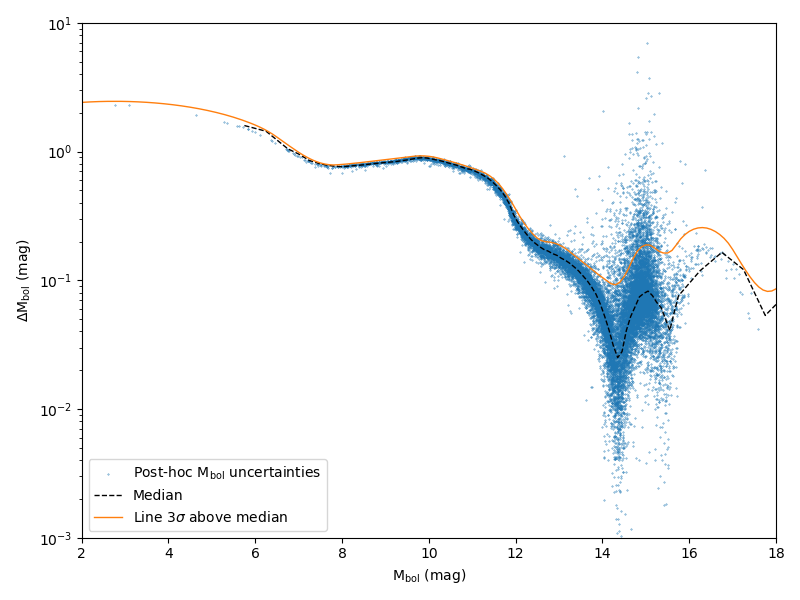
\includegraphics[width=\columnwidth]{figures/fig_03_mbol_sigma.png}
    \caption{Caption}
    \label{fig:mbol_sigma}
\end{figure}

\begin{figure}
    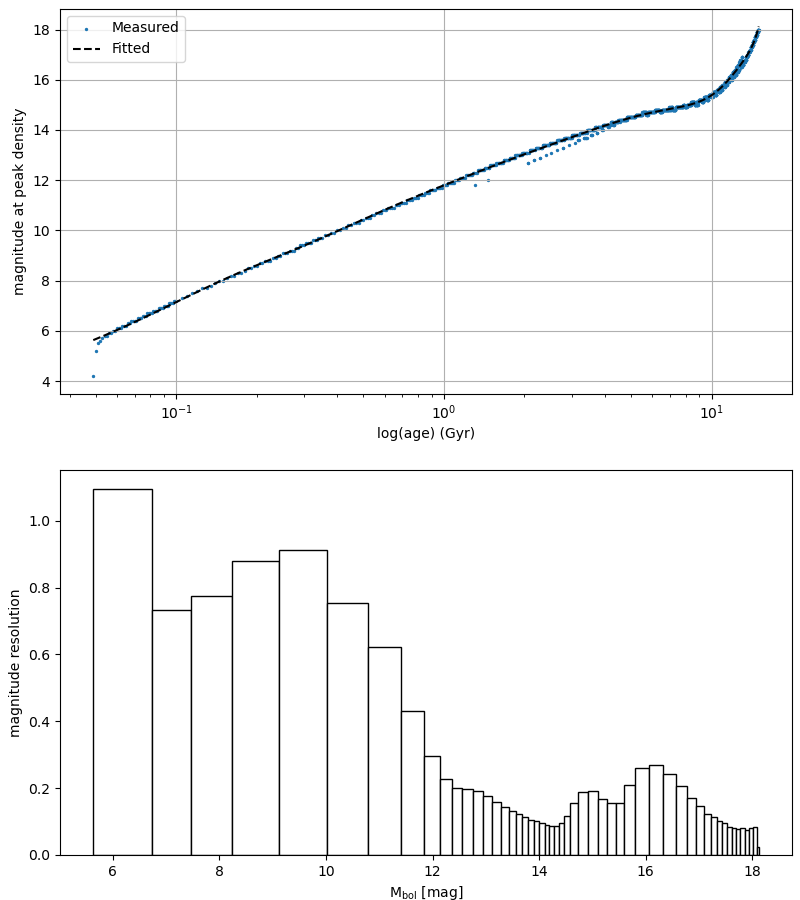
\includegraphics[width=\columnwidth]{figures/fig_04_magnitude_resoltuion.png}
    \caption{Caption}
    \label{fig:magnitude_resolution}
\end{figure}

\begin{figure}
    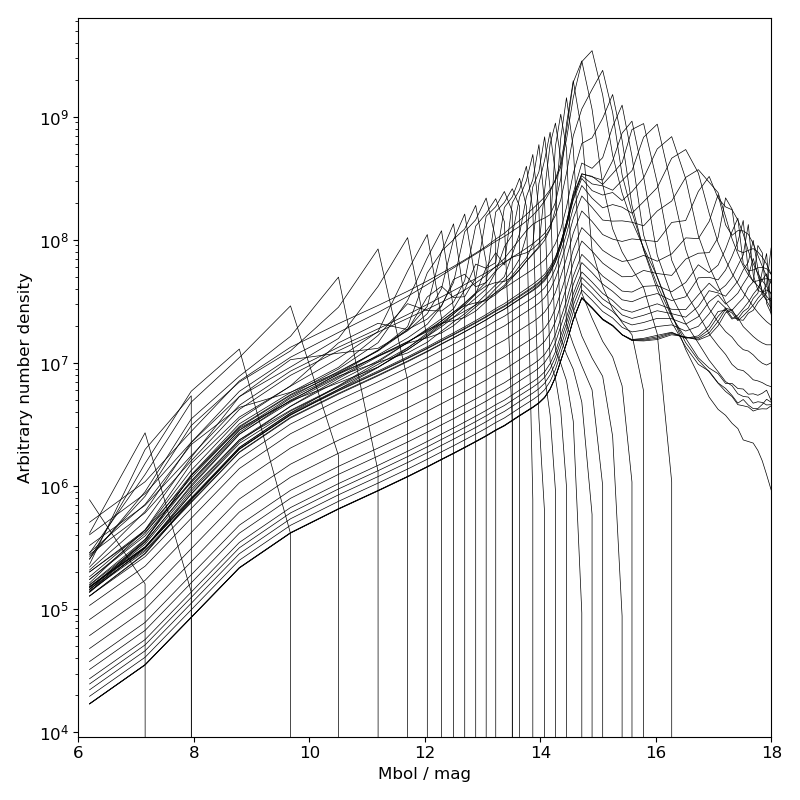
\includegraphics[width=\columnwidth]{figures/fig_05_basis_pwdlf.png}
    \caption{The set of partial WDLF (basis functions) that the peaks are separated by the magnitude resolution as found in Fig~\ref{fig:magnitude_resolution}.}
    \label{fig:basis_pwdlf}
\end{figure}

\subsection{Star Formation History}

\begin{figure*}
    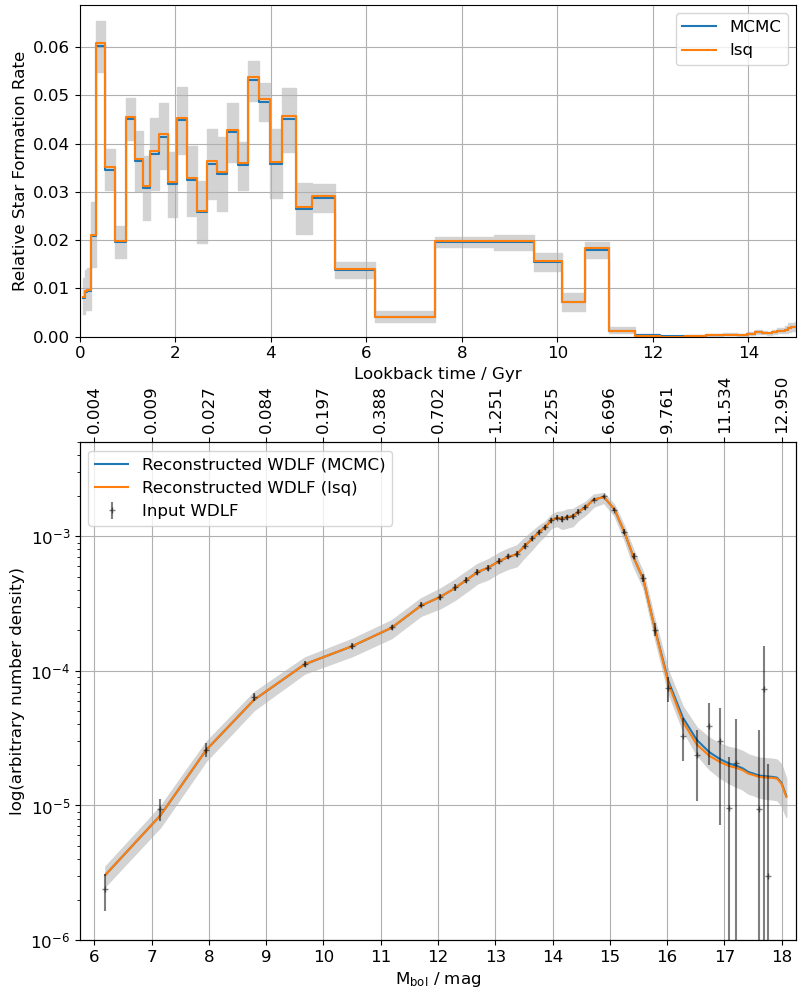
\includegraphics[width=\textwidth]{figures/fig_06_gcns_reconstructed_wdlf_optimal_resolution_bin_optimal.png}
    \caption{Top: The weights of the pWDLFs found from MCMC sampling finished with a least-squares minimisation. Bottom: the reconstructed WDLF using the pWDLFs.}
    \label{fig:sfh_mag_bin_05}
\end{figure*}



\subsection{Comparison with previous studies}

\begin{figure}
  \dummyfig{Comparison} 
  \caption{Compared against previous works. red hue dashed lines show the SFH based on WD. blue hur dotted lines show the SFH found using other stellar populations.}
  \label{fig:dummy3}
\end{figure}


\section{Conclusions and Future Work}
Historically, all the luminosity functions of the solar neighbourhood were reported
in the bolometric magnitudes. Essentially, all works were reporting the
WD-Bolometric-LF. To address the problem of degeneracy in the solution, we explore
the use of colour information from the luminosity function, where we are using
the WDLF in multiple filters . 



\section*{Acknowledgements}


%%%%%%%%%%%%%%%%%%%%%%%%%%%%%%%%%%%%%%%%%%%%%%%%%%
\section*{Data Availability}


%%%%%%%%%%%%%%%%%%%% REFERENCES %%%%%%%%%%%%%%%%%%

% The best way to enter references is to use BibTeX:

\bibliographystyle{mnras}
\bibliography{sfh_wd} % if your bibtex file is called example.bib


% Alternatively you could enter them by hand, like this:
% This method is tedious and prone to error if you have lots of references
%\begin{thebibliography}{99}
%\bibitem[\protect\citeauthoryear{Author}{2012}]{Author2012}
%Author A.~N., 2013, Journal of Improbable Astronomy, 1, 1
%\bibitem[\protect\citeauthoryear{Others}{2013}]{Others2013}
%Others S., 2012, Journal of Interesting Stuff, 17, 198
%\end{thebibliography}

%%%%%%%%%%%%%%%%%%%%%%%%%%%%%%%%%%%%%%%%%%%%%%%%%%

%%%%%%%%%%%%%%%%% APPENDICES %%%%%%%%%%%%%%%%%%%%%

\appendix

\section{Some extra material}

%%%%%%%%%%%%%%%%%%%%%%%%%%%%%%%%%%%%%%%%%%%%%%%%%%


% Don't change these lines
\bsp	% typesetting comment
\label{lastpage}
\end{document}

% End of mnras_template.tex
